\documentclass[tikz,border=10pt]{standalone}
\usepackage{tikz}
\usetikzlibrary{calc}
\begin{document}
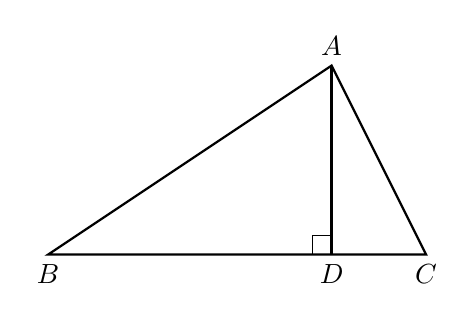
\begin{tikzpicture}[scale=1.2, >=stealth]    
% 1. 定义关键点坐标    
% 设定 D 为原点，根据原图比例设定 A, B, C 的相对位置    
\coordinate (D) at (0,0);    
\coordinate (A) at (0,2);      % 顶点 A 在 D 正上方    
\coordinate (B) at (-3,0);     % B 点在左侧，距离较远    
\coordinate (C) at (1,0);      % C 点在右侧，距离较近
    % 2. 绘制三角形主体和高线    
\draw[thick] (A) -- (B) -- (C) -- cycle; % 绘制三角形 ABC    
\draw[thick] (A) -- (D);                 % 绘制高线 AD
    % 3. 绘制直角符号 (Right angle mark at D)    
% 尺寸设为 0.2 单位    
\draw (D) ++(-0.2,0) -- ++(0,0.2) -- ++(0.2,0);
    % 4. 标注顶点文字    
% 使用 anchor 确保文字不遮挡线条    
\node[above] at (A) {$A$};    
\node[below] at (B) {$B$};    
\node[below] at (C) {$C$};    
\node[below] at (D) {$D$};
\end{tikzpicture}
\end{document}